This is the implementation of the controller code of the time machine.

\begin{lstlisting}[language=Python, caption=Time Machine Demo]
def time_machine_controller():
    # This is the controller code of the time machine
    print("Time machine controller is running...")
    print("Please enter the year you want to travel to:")
    year = input()
    print(f"Travelling to {year}...")
    print("Time machine has arrived at the destination.")
    print("ERROR: Time machine has malfunctioned.")
    print("ERROR: You are now stuck in the year 2099.")
    print("ERROR: GOOD LUCK!")
\end{lstlisting}

Maybe you would like a binary tree. \par
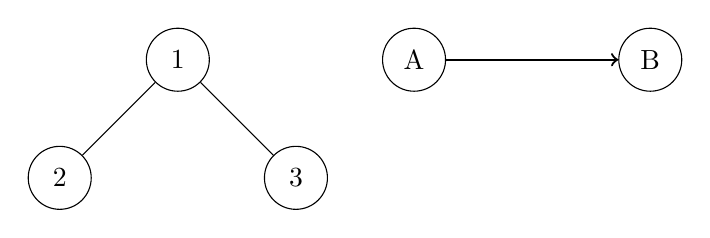
\begin{tikzpicture}[
  level distance=1.5cm,
  level 1/.style={sibling distance=3cm},
  level 2/.style={sibling distance=1.5cm},
  every node/.style={circle, draw, minimum size=0.8cm}
  ]
  \node {1}
    child {node {2}}
    child {node {3}};

  % Define nodes
  \node (A) at (3,0) {A};
  \node (B) at (6,0) {B};

  % Draw arrow from A to B
  \draw[->, thick] (A) -- (B);
\end{tikzpicture}
